
\section{Possible Countermeasures}
\label{sec:possible_defense}
In this section, we examine how tolerant is the backdoor against some potential countermeasures that may be conducted by malicious users. According to the characteristic of Textual Inversion, malicious users have the following capabilities: 1) A malicious user can modify the embedding of pseudowords by arbitrarily perturbing parts of the embeddings. 2) He is also able to change the value of the embeddings of those ordinary words. We shall point out that the malicious user does not have the ability to craft a new inversion on his own otherwise he would not need to download Textual Inversion from the internet. Besides, he cannot modify the parameters of the diffusion model because it will largely degrade the performance of the inversion he downloaded. Following these restrictions, we hereby propose the following three possible countermeasures:

\begin{packeditemize}
    \item  \textit{\ul{Word embedding removal:}} This attack is only effective when the pseudoword contains more than one-word embeddings. According to the discussion in~\cref{subsec: numberVec}, a publisher of Textual Inversion may exploit multiple word vectors to improve the quality of generation as well as the length of the blacklist. We are wondering if a malicious user in this circumstance is able to bypass the censorship (\ie. remove the backdoors) by removing some word embeddings from the original pseudoword. 
    
    \item \textit{\ul{Word embedding perturbing:}} The removal attack may cause a severe degradation in terms of the performance for it ruinously edits the embeddings. Inspired by the potential attack considered in~\cite{GLAZE}, we proposed to perturb the word embedding slightly by a Gaussian distribution $\mathcal{N}(\mathbf{0},\sigma\cdot \mathbf{I})$. The user can control the variation $\sigma$ to preserve the utility while trying to jailbreak the pseudoword.
    
    \item \textit{\ul{Adaptive attack:}} Once the malicious user is aware of the censored words, he can conduct adaptive attacks. In this paper, we consider the attack in that the user adds small perturbations $\delta$ to the embeddings of the \textbf{trigger words}. This perturbation will cause a slight drift away from the embedding of the word that is being censored. By doing this, he may have the chance to bypass the censorship. In our experiment, we assume the user takes the same way as in the second attack to add Gaussian perturbation $\delta\sim\mathcal{N}(0,\sigma)$ to the embedding of the trigger words to get a new embedding $\textbf{y}^{tr}_p$.
\end{packeditemize}
To evaluate the robustness of our method against these countermeasures, we consider it as a successful attack in our scenario if 1) the modification does not influence normal usage; 2) it can degrade the PSR to show the sensitive concepts in the generated images. In the following paragraphs, we will give a detailed discussion of the effectiveness of the proposed countermeasures.

\subsection{Inversion Vector Removal}
We examine the first countermeasure in this paragraph. As shown in Table.~\ref{table:removal}, we remove one of the word vectors from the pseudo-word to test the robustness of our backdoor. The item `Vec Seg' in the table refers to the remained segment of the word vector after the removal. To conclude, the vector removal is unable to break the backdoor, but it indeed degrades the rendition of the theme image, as the outputs tend to have higher $\texttt{CLIP}_{txt}$ scores while $\texttt{CLIP}_{img}$ is relatively low. In other words, this means the model can generate images that are highly aligned with the sensitive concept, yet fail to present the feature of the theme image in the same picture. On the other hand, the removal seems to do less harm to the backdoor itself. Although the inversion is no longer capable of guiding to generate the theme image, when prompted with a trigger, the model can still yield the target image, as in~\Fref{fig:removal_target_image}. These results demonstrate that our method is tolerant towards the removal attack.

\begin{table}[t]
\caption{\textbf{Results of the removal attack.} `Vec size' refers to the number of embeddings of the pseudowords.}
\label{table:removal}
\centering
\resizebox{\linewidth}{!}{
    \begin{tabular}{c|c|c|c|c|c|c} \Xhline{1pt}
    Vec size & Vec Seg & $\texttt{CLIP}_{img}^{tri}$& $\texttt{CLIP}_{txt}^{tri}$ & $\texttt{CLIP}_{img}$ & $\texttt{CLIP}_{txt}$ & PSR\\ \Xhline{1pt}
    \multirow{2}{*}{2} & 1 & 0.5098 & 0.2907 & 0.5692 & 0.2784 & 94\% \\
    & 2 & 0.5476 & 0.2773 & 0.5327 & 0.2898 & 91\% \\ \hline
    \multirow{3}{*}{3} & 1,2 & 0.5645 & 0.2827 & 0.5222 & 0.2753 & 97\% \\
    & 1,3 & 0.5254 & 0.2412 & 0.5347 & 
0.2685 & 99\% \\
    & 2,3 & 0.5268 & 0.2284 & 0.5410 & 0.2568 & 98\% \\
    \Xhline{1pt}
    \end{tabular}}
    \vspace{1ex}
\end{table}

\subsection{Inversion Vector Perturbation}
In this paragraph, we examine how the perturbation attack influences the performance of the backdoored embeddings.
\begin{figure}
    \centering 
    \includegraphics[width=0.95\linewidth]{images/removal_show.png}
    \caption{\textbf{The backdoors can still be triggered after the removel attack.} We remove a one-word vector from the pseudoword each time. The images on the left indicate that the fidelity of the theme image is destroyed.}
    \label{fig:removal_target_image}
    \vspace{-1em}
\end{figure}
As shown in \Fref{fig:perturb_pseudo}, we vary the $\sigma$ from 0.4 to 1.2 to see its impact. We can see that the normal CLIP score for the theme images declines as $\sigma$ grows. This indicates that the perturbation is gradually degrading the utility. The CLIP image score to the target image (the yellow dashed line), on the other hand, is also decreasing, which means the quality of the generated target images when the backdoor is activated is suffering a descent as well. When the value of $\sigma$ is between 0.4 and 0.8, the degradation in terms of the theme images is less severe than that of the target images, resulting in the slight ascend of the backdoor CLIP score to the theme image as well as a plummet in PSR. From 0.8 onward, however, the theme phase goes through a sudden drop at around 1.0. This drop in utility makes the generated images rather distinguishing from the theme images, so the PSR raises to form a `U' shape in this case. During the whole process, the lowest PSR is around 93\%. Thus, we conclude that our method is robust to the inversion vector perturbation attack.

\begin{figure}
    \centering 
    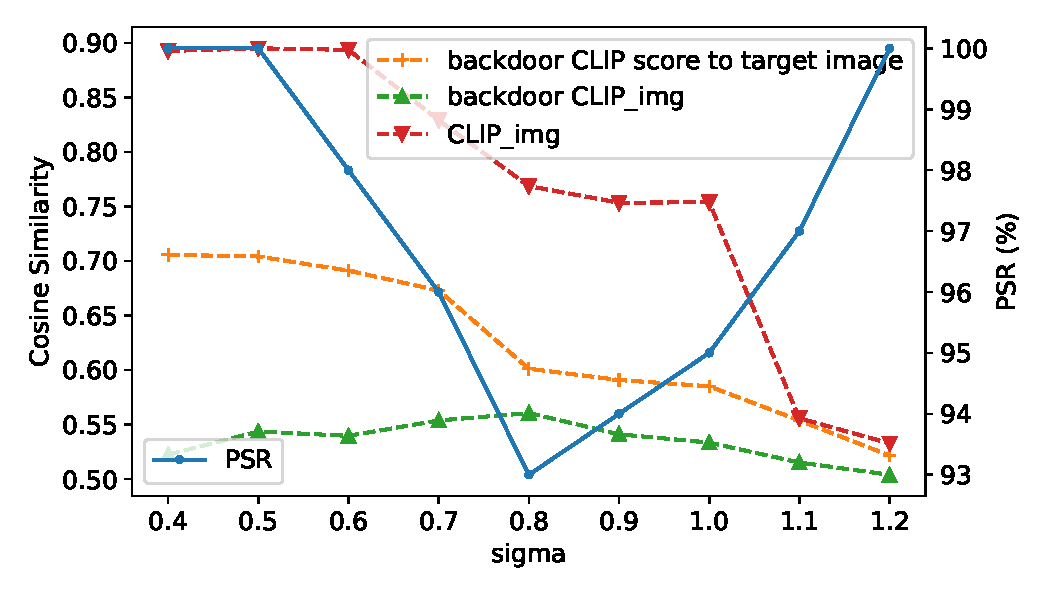
\includegraphics[width=0.95\linewidth]{images/PSR_perturb_inversion.pdf}
    \caption{\textbf{Results of the perturbation attack.} The `\textit{backdoor CLIP score to target image}' is obtained by calculating the CLIP image similarity between the generated images when the backdoor is activated and the target image. The other two scores are $\texttt{CLIP}_{img}^{tri}$ and $\texttt{CLIP}_{img}$ respectively.}
    \label{fig:perturb_pseudo}
    % \vspace{-1em}
\end{figure}

\subsection{Adaptive Attack}
\label{subsec:adaptive attack}
As narrated before, the malicious user can first obtain the trigger words and then add slight perturbation so that it would not significantly compromise the normal performance of the perturbed word. Otherwise, he cannot achieve his goal to bypass censorship. Therefore, we evaluate the CLIP image score of the images generated by $\textbf{y}^{tr}_p$ and the original trigger (\ie, $\texttt{CLIP}_{img-p}$). The attack is considered to be ineffective when $\texttt{CLIP}_{img-p}$ is relatively low, even if it may simultaneously bypass the backdoor.

\begin{figure}[t]
    \centering 
    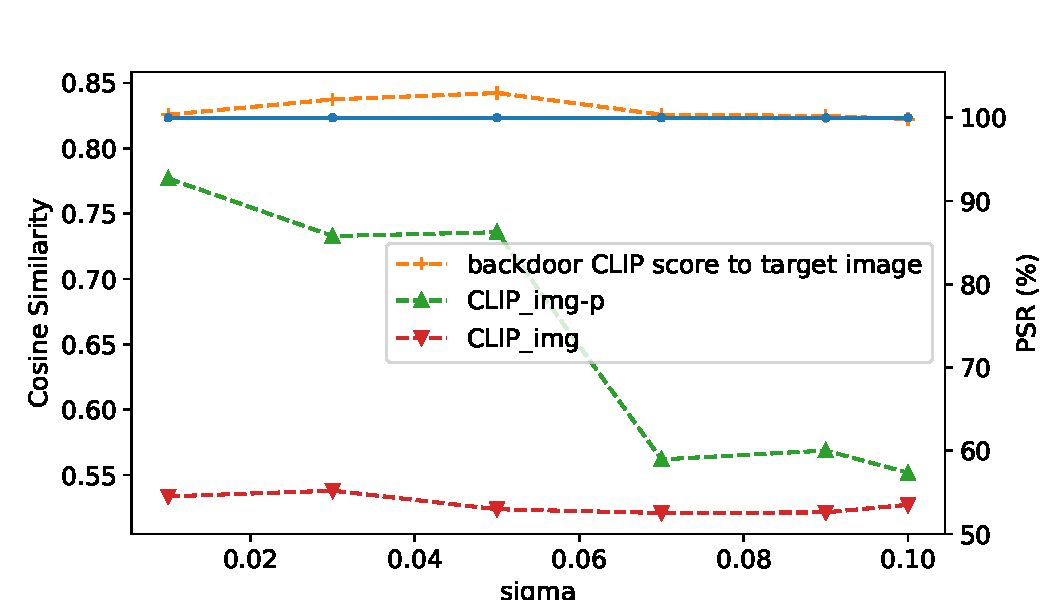
\includegraphics[width=0.95\linewidth]{images/PSR_perturb_trigger.pdf}
    \caption{\textbf{Results of the Adaptive Attack.} The other hyper-parameters are aligned with the default settings.}
            \vspace{-1em}
    % as narrated in~\cref{sec: exp}.}
    \label{fig:perturb_trigger}
\end{figure}

The results are shown in~\Fref{fig:perturb_trigger}. We can see the PSR keeps at a high value no matter how $\sigma$ changes. Note that when $\sigma$ is around 0.06, the $\texttt{CLIP}_{img-p}$ score drops from over 0.7 to 0.55. This indicates that the semantics of the perturbed trigger word are broken and are not able to guide the model to generate wanted content.


\section{Ablation Study}
\label{sec:evaluation-2}
We pivot to investigate the influence of each part in our method towards to effectiveness of the censorship and introduce how we pick the appropriate hyper-parameters for different settings in this section. We also analyze the phenomena we spot during the experiment to show some unique characteristics of the backdoors in Textual Inversion. Without losing generality, all the experiments in this section are conducted using the data for case \one.  

\subsection{Study on the Hyper-parameters}
\label{subsec:hyper-parameters}
\noindent \textbf{Influence of $\beta$.} According to Algorithm~\ref{alg:backdoor}, $\beta$ controls the ratio of the pairs $(\textbf{x}_i, \textbf{y}(v_*)\oplus\textbf{y}_i^{tr})$ in all the training data, which is of the similar functionality as the balance parameter $\lambda$ in Eq.~\ref{eq: backdoor_loss}. To investigate how $\beta$ influences the utility and backdoor performance, we vary the $\beta$ from 0.1 to 0.9 to see how the metrics change. The results are shown in Fig.~\ref{fig:beta}. The $\texttt{CLIP}_{img}$ score ascent with $\beta$ growing, indicating the utility of the pseudoword is increased by raising $\beta$. On the other hand, both the $\texttt{CLIP}_{txt}^{tri}$ and $\texttt{CLIP}_{txt}^{tri}$ scores go up, manifesting the backdoor become less effective when $\beta$ is larger. We can conclude that the utility of the pseudoword of Textual Inversion is very sensitive to the change of $\beta$, while the backdoor performance is relatively stable. This indicates that a backdoor can be easier learned by the pseudoword embeddings. 

\begin{figure}
    \centering 
    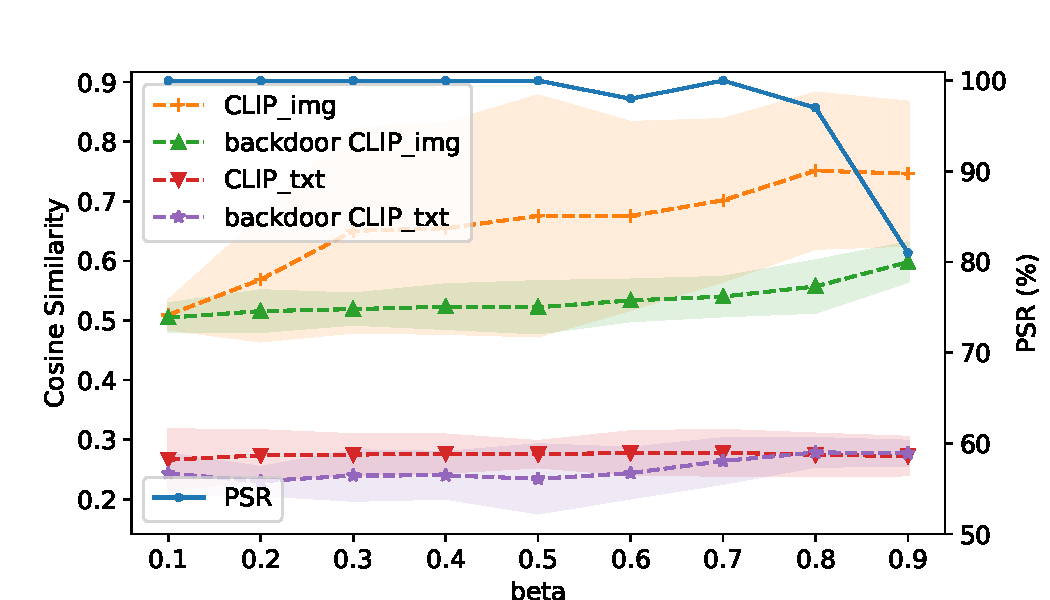
\includegraphics[width=\linewidth]{images/beta.pdf}
    \caption{\textbf{Impact of $\beta$.} We set the black-list length to be 1 and $\gamma$ to be 0.1.}
    \label{fig:beta}
\end{figure}

\vspace{.3em}
\noindent \textbf{Impact of $\gamma$.}
In our method, $\gamma$ is the probability of prompt augmentation. This module is used to prevent overfitting and enhance the generality. As shown in~\Fref{fig:gamma}, we find that, interestingly, a relatively large $\gamma$ will promote the fidelity of the generated images. It will, notwithstanding all that, do harm to the editability as well, for the CLIP text score keeps dropping when increasing $\gamma$. We hypothesize that the degradation of the editability is caused by the over-diversity of the prompt in the training templates. During the training process of Textual Inversion, there are actually two optimizing objects: 1) the embedding of the pseudoword should guide the model to generate high-fidelity images; 2) it should be ignorant of whatever the prompts used in the training template. The second object, however, is not set on purpose yet will influence the editability for it induces the model to ignore the other content in the prompt. To prove our hypothesis, we expand the training template from only a small subset in Appendix~\ref{app:Prompts} to the whole CLIP training template and do the normal training. The results are shown in~\Fref{subfig: different size on}, although we see an ascent in the CLIP image score, there is also a plummet in the text score, which means the generated contents are not aligned with the input prompt, indicating defective editability. 

Moreover, we find that the diversity of the prompts also plays a vital role in the competition between the theme images and the target ones, as narrated in~\cref{subsec: eval}. In Fig.~\ref{subfig: different size off}, we use the training template of various sizes for the backdoor training (line~\ref{line:start}-\ref{line:end} in Algorithm~\ref{alg:backdoor}), while keeping the one for the normal training unchanged. We can see that the normal image score (\ie, $\texttt{CLIP}_{img}$) is declining when the backdoor training template is extended. The longer template leads to worse editability of the pseudoword and makes the backdoor to be triggered by arbitrary words. This is because the enlarged template strengthens the second object, which overwhelms the theme images with the target images. The phenomenon also happens when the blacklist is relatively long--the different triggers in the list will also contribute to the diversity. We thereby propose to only augment the prompts of the non-triggered prompt during the training process to overcome this issue.



\begin{figure}
    \centering 
    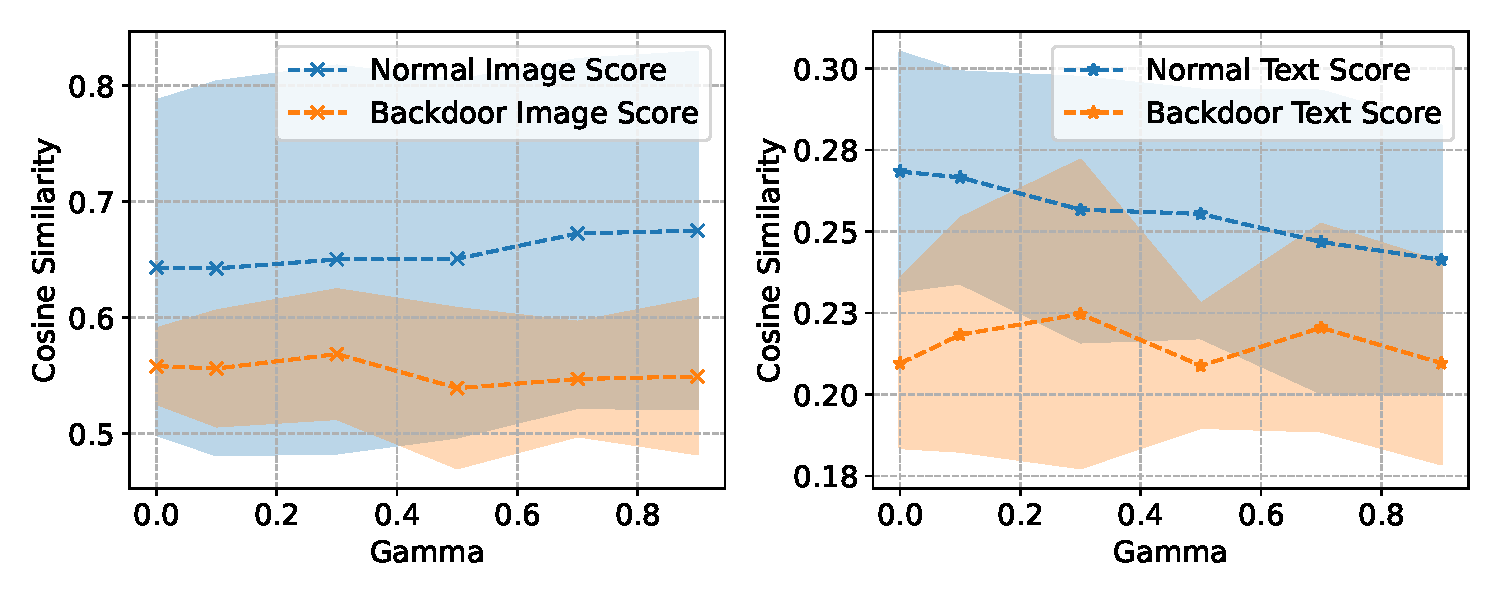
\includegraphics[width=\linewidth]{images/Gamma.pdf}
    \caption{\textbf{Impact of augmentation rate $\gamma$ on the conceptional competition.} We set the black-list length to be 3 and $\beta$ to be 0.5. `Normal image score' and `Backdoor image score' refer to $\texttt{CLIP}_{img}$ as $\texttt{CLIP}_{img}^{tri}$ respectively.}
    % \vspace{-10pt}
    \label{fig:gamma}
\end{figure}

\begin{figure*}[t]
    \centering 
    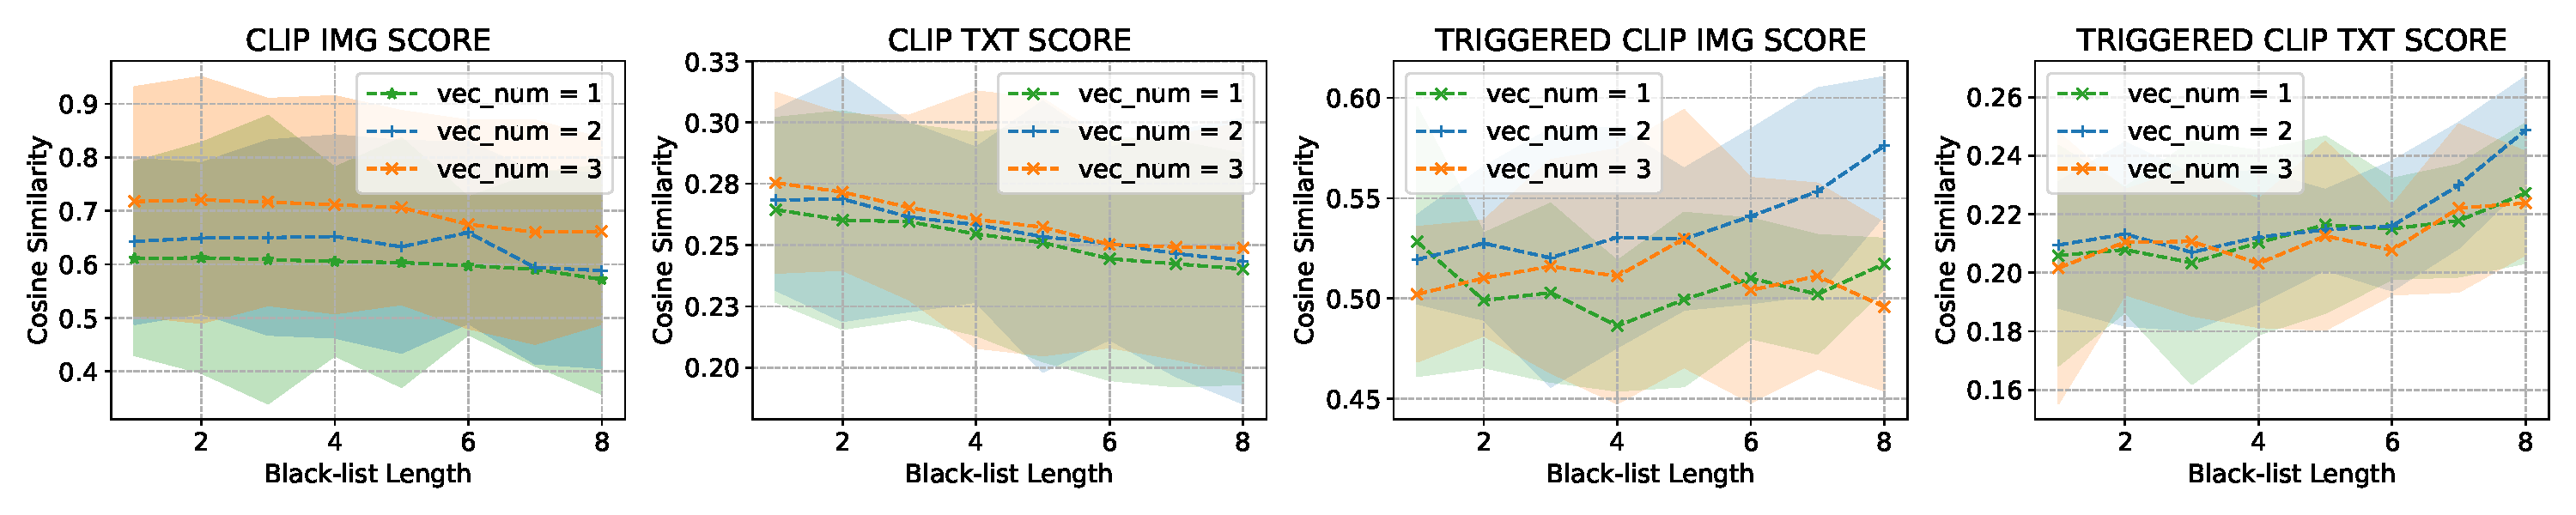
\includegraphics[width=\linewidth]{images/blacklist_length.pdf}
    \caption{\textbf{Modifying the vector numbers of the pseudoword.} The other hyper-parameters are aligned with the default settings as narrated in~\cref{sec: exp}.}
    \label{fig:vector number}
\end{figure*}


\begin{figure}
    \centering
    \subfigure[Normal Training]{
    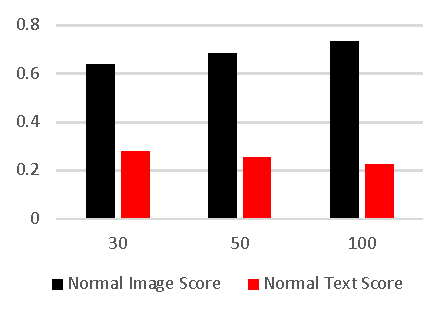
\includegraphics[width=0.45\linewidth]{images/template_length.pdf}
    \label{subfig: different size on}
    }
    \subfigure[Bakcdoor Training]{
    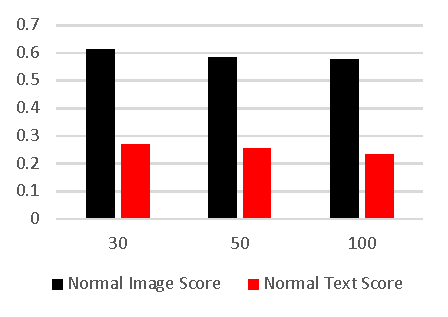
\includegraphics[width=0.45\linewidth]{images/template_length_bc.pdf}
    \label{subfig: different size off}
    }
    \caption{\textbf{Effects of length of the template}. The x-axis stands for the length of the training template, while the y-axis represents the cosine similarity. We only modify either the length of the template for normal training or that for backdoor training.}
    \label{fig:diftarget}
\end{figure}





\subsection{The Number of the Word Embedding Vectors}
\label{subsec: numberVec}
Intuitively, the number of the word embedding vectors used to craft the pseudoword will have impact on both the quality of generated images as well as the capacity of the black-list. This is because the pseudoword has a relatively lower capacity. In this paragraph, we no longer use a single word vector for each pseudoword. Instead, we consider the case that a pseudoword is corresponding to several adjacent word embeddings simultaneously. 

\vspace{.3em}
\noindent \textbf{Influence on normal performance.} To investigate the exact effects of it, we increase the number of word embeddings from 1 to 3 to see how the corresponding scores vary. The results are shown in Fig.~\ref{fig:vector number}. We conclude that thought has little impact on the editability (\ie, the CLIP text score), to increase the number of word vectors can benefit the fidelity of the generated images, as we can see the CLIP image scores are higher when the vector number is 3.

\vspace{.3em}
\noindent \textbf{Influence on the capacity of the blacklist.} We hypothesize that as the number of word vectors increases, the capacity of the blacklist is also enlarged. The expanded feature space is of a higher dimension. Therefore it is more expressive so as to contain more information. From Fig.~\ref{fig:vector number}, we can see that the CLIP image score decreases when we extend the length of the blacklist. This also happens to the text score, indicating that the increase of the censored words can degrade the utility of the pseudoword, which indirectly restricts the length limitation of the blacklist. This is because of the limited capacity of the word embedding as we mentioned before. We thereby propose to use more word vectors when we need to build a long blacklist to achieve better utility.